\section{Longitudinal Vehicle Model}
\label{longitudinal_vehicle_model}

In this section, we will develop a longitudinal vehicle model using the  \lstinline{chronos}.
(see \url{http://projectchrono.org/})



\subsection{Setup the Vehicle}

Our vehicle will be represented by the \lstinline{Vehicle} class. This class wraps the following information for us

\begin{itemize}
\item \lstinline{std::shared_ptr<chrono::ChSystem> system_}
\item \lstinline{std::shared_ptr<vehicle_t> vehicle_}
\item \lstinline{std::shared_ptr<powertrain_t> powertrain_}
\item \lstinline{chrono::ChMaterialSurface::ContactMethod contact_method_}
\item \lstinline{chrono::vehicle::TireModelType tire_type_}
\item \lstinline{chrono::ChCoordsys<> init_pos_}
\item \lstinline{bool is_fixed_}
\item \lstinline{bool apply_drag_}
\item \lstinline{std::vector<double> init_omega_}
\item \lstinline{std::array<chrono::vehicle::ChTire*, 4> tires_}
\item \lstinline{std::map<std::string, double> properties_}
\end{itemize}


Every simulation must have a \lstinline{Vehicle}


\subsection{Setup the Terrain}


\subsection{Setup the Simulation Application}


\subsection{Simulation Results}

 
Specifically, we will simulate a vehicle that moves in straight line.  Figure \ref{straight_line_motion} shows a snapshot of the simulation

\begin{figure}[!htb]
\begin{center}
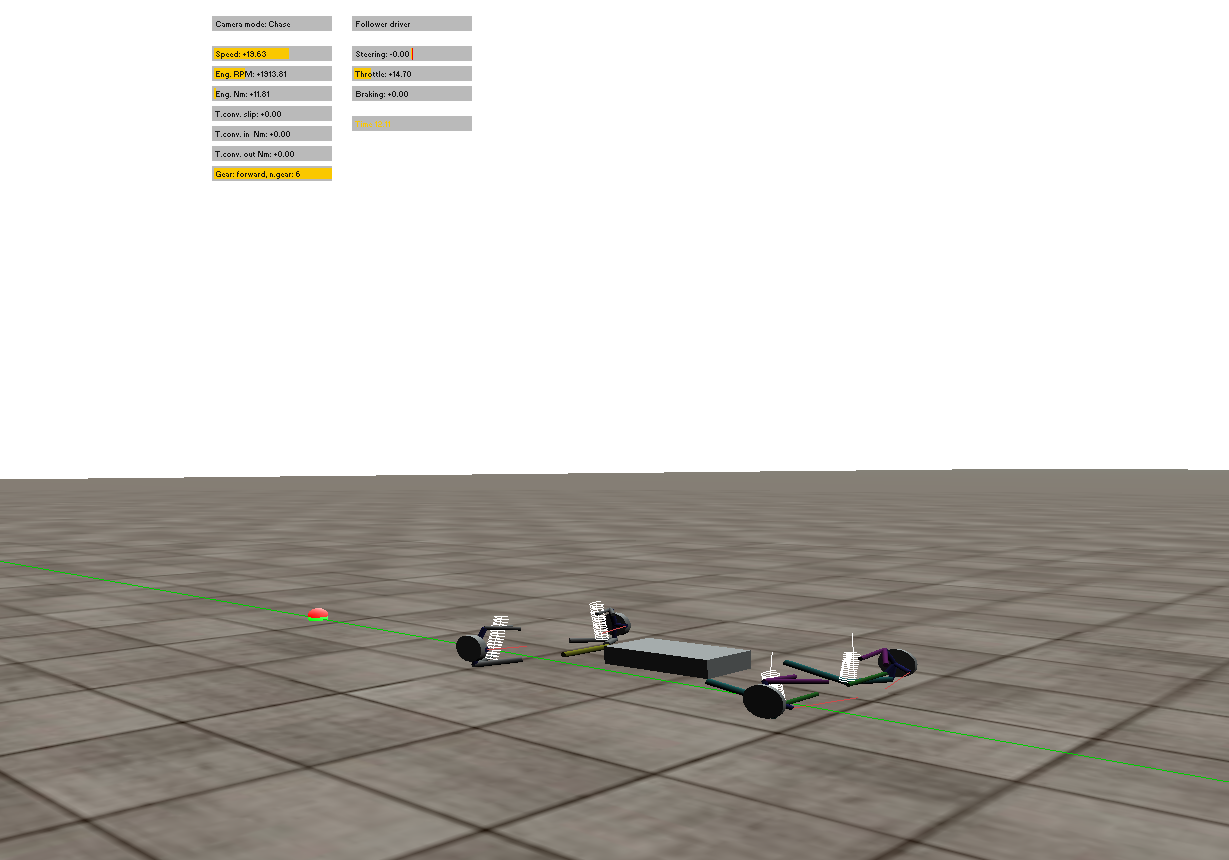
\includegraphics[scale=0.290]{img/straight_line_motion.png}
\end{center}
\caption{Straight line vehicle motion.}
\label{straight_line_motion}
\end{figure}

See \url{http://api.projectchrono.org/tutorial_install_project.html} for further information. The reference manual can be found at
\url{http://api.projectchrono.org/manual_root.html}.

\subsection{The \lstinline{Chrono::Vehicle} library}

The \lstinline{Chrono::Vehicle} is a C++ middleware library for the modeling, simulation, and visualization of wheeled and tracked ground vehicles.
It consists of two core modules:

\begin{itemize}
\item The \lstinline{ChronoEngine_vehicle}

	\begin{itemize}
		\item Defines the system and subsystem base classes
		\item Provides concrete, derived classes for instantiating templates from JSON specification files
		\item Provides miscellaneous utility classes and free functions for file I/O, Irrlicht vehicle visualization, steering and speed controllers, vehicle and subsystem test rigs, etc.
	\end{itemize}

\item The \lstinline{ChronoModels_vehicle}
	\begin{itemize}
		\item Provides concrete classes for instantiating templates to model specific vehicle models
	\end{itemize}
\end{itemize}

The following dependencies should be satisfied in order to use the library.

\begin{itemize}
\item The \lstinline{Chrono::Engine } required
\item The \lstinline{Chrono::Irrlicht} and the \lstinline{Irrlicht} library,  \lstinline{Chrono::OpenGL} and its dependencies. Both are optional
\item The \lstinline{Chrono::FEA} and \lstinline{Chrono::MKL} (optional)
\end{itemize}

The \lstinline{Chrono::Engine } supports the notion of a system. In our case, the following components are considered a system

\begin{itemize}
\item Powertrain
\item Tire
\item Terrain
\item Driver
\item Vehicle
\end{itemize}

\lstinline{Chrono::Vehicle} encapsulates templates for systems and subsystems in polymorphic C++ classes:

\begin{itemize}
\item A base abstract class for the system/subsystem type (e.g. \lstinline{Chrono::ChSuspension})
\item A derived, still abstract class for the system/subsystem template (e.g.  \lstinline{Chrono::ChDoubleWishbone})
\item Concrete class that particularize a given system/subsystem template (e.g. \lstinline{Chrono::HMMWV_DoubleWishboneFront})
\end{itemize}

\subsection{The \lstinline{chrono::vehicle::ChVehicle} class}

Vehicles in \lstinline{Chrono} inherit from the base class \lstinline{chrono::vehicle::ChVehicle}. 
This class provides the interface between the vehicle system and other systems (tires, driver, etc.)

The reference frame for a vehicle follows the ISO standard. 
Namely, $Z$-axis up, $X$-axis pointing forward, and $Y$-axis towards the left of the vehicle. The following figure illustrates
the asseumed reference frames.


\begin{figure}[!htb]
\begin{center}
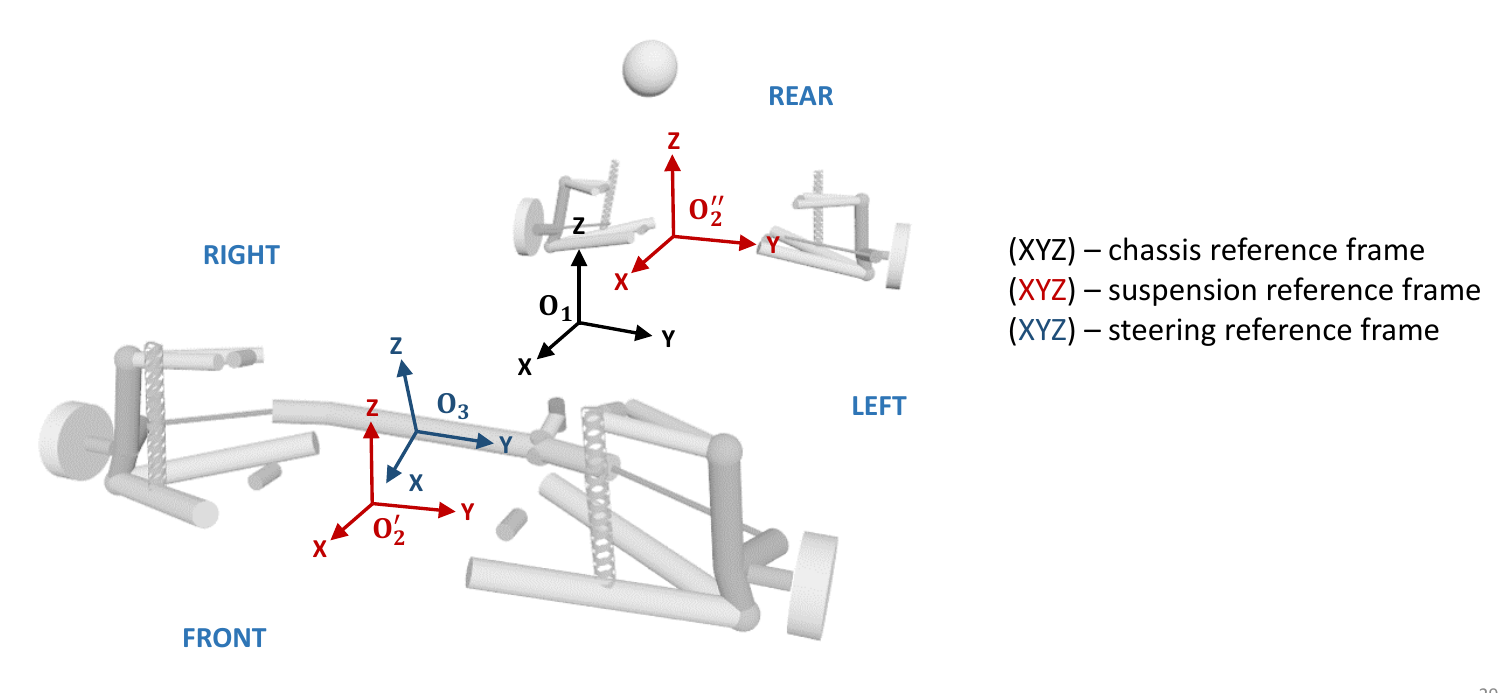
\includegraphics[scale=0.290]{img/vehicle_iso_ref_frame.jpeg}
\end{center}
\caption{Vehicle ISO reference frames.}
\label{vehicle_iso_ref_frame}
\end{figure}

A \lstinline{chrono::vehicle::ChVehicle} has

\begin{itemize}
\item \lstinline{ChSystem* m_system} pointer to the Chrono system
\item \lstinline{std::shared_ptr<ChChassis> m_chassis} handle to the chassis subsystem
\item \lstinline{bool m_ownsSystem} true if system created at construction
\item \lstinline{double m_stepsize}  integration step-size for the vehicle system
\end{itemize}

Deferring to its constituent subsystems as needed, a \lstinline{chrono::vehicle::ChVehicle} provides accessors for:

\begin{itemize}
\item Underlying \lstinline{chrono::vehicle::ChSystem}
\item Handle to the vehicle chassis
\item Chassis state (reference frame and COM)
\item Angular speed of the vehicle driveshaft (connection to powertrain)
\end{itemize}

A \lstinline{chrono::vehicle::ChVehicle} intermediates communication between other systems (e.g.,
powertrain, driver, etc.) and constituent subsystems (e.g., suspensions, brakes, etc.)

\subsection{ The \lstinline{chrono::vehicle::ChChassis} class}

This is the ase class for the chassis vehicle subsystem. The class documentation can be found at 
\url{http://api.projectchrono.org/classchrono_1_1vehicle_1_1_ch_chassis.html}. A chassis has the following attributes

\begin{itemize}
\item \lstinline{std::shared_ptr<ChBodyAuxRef> m_body}; a handle to the chassis body
\item \lstinline{bool m_fixed}; a flag indicating if the chassis body is fixed to the ground
\end{itemize}

It provides access to the following properties

\begin{itemize}
\item Chassis mass and inertia properties
\item Chassis state reference frame and COM
\item Vehicle speed reference frame and COM
\item Driver position
\item Absolute acceleration of a point specified in local reference frame
\end{itemize}

A chassis system can be specified in a JSON file.

\subsection{ The \lstinline{chrono::vehicle::ChDriver} class}

Base class for a vehicle driver system.
A driver system must be able to report the current values of the inputs (throttle, steering, braking). 
A concrete driver class must set the member variables:

\begin{itemize}
\item \lstinline{m_throttle}
\item \lstinline{m_steering} 
\item \lstinline{m_braking}
\end{itemize}
Since these are the main quantities that a driver can interact with a vehicle, this class has to be adapted
when we want to incorporate autonomy. 


\subsection{Setup simulation}

In order to set up our simulation, we need to establish the following

\begin{itemize}
\item Powertrain
\item Tire
\item Terrain
\item Driver
\item Vehicle
\end{itemize}

We will see further below how to create these systems. First however let's introduce some constants we will be using in the simulation.


\begin{lstlisting}
#include "chrono/core/ChFileutils.h"
#include "chrono/core/ChRealtimeStep.h"
#include "chrono/utils/ChFilters.h"

#include "chrono_vehicle/ChVehicleModelData.h"
#include "chrono_vehicle/terrain/RigidTerrain.h"
#include "chrono_vehicle/driver/ChIrrGuiDriver.h"
#include "chrono_vehicle/driver/ChPathFollowerDriver.h"
#include "chrono_vehicle/utils/ChVehiclePath.h"
#include "chrono_vehicle/wheeled_vehicle/utils/ChWheeledVehicleIrrApp.h"
\end{lstlisting}

\begin{lstlisting}


using namespace chrono;
using namespace chrono::geometry;
using namespace chrono::vehicle;

namespace demo_data
{

    const std::string BASIC_DATA_PATH("/home/david/MyProjects/cubic_engine/chrono_lib/chrono/data/vehicle/paths/");

    // Rigid terrain dimensions
    const double TERRAIN_HEIGHT = 0;
    const double TERRAIN_LENGTH = 300.0;  // size in X direction
    const double TERRAIN_WIDTH = 300.0;   // size in Y direction
    const std::string TERRAIN_PATH("/home/david/MyProjects/cubic_engine/chrono_lib/chrono/data/vehicle/terrain/textures/tile4.jpg");

    // Input file names for the path-follower driver model
    const std::string PATH_FILE(BASIC_DATA_PATH + "straight.txt");

    // Initial vehicle location and orientation
    const ChVector<> INIT_LOC(-125, -125, 0.5);
    const ChQuaternion<> INIT_ROT(1, 0, 0, 0);

    // Desired vehicle speed (m/s)
    double target_speed = 20;

    // Point on chassis tracked by the chase camera
    const ChVector<> TRACK_POINT(0.0, 0.0, 1.75);

    // Simulation step size
    const double DELTA_T = 2e-3;
    const double TIRE_DELTA_T = 1e-3;

    // Simulation end time
    const double TIME_END = 100;

    // Render FPS
    const double FPS = 60;

    // Debug logging
    const bool DEBUG_OUTPUT = false;
    const double DEBUG_FPS = 10;

    // Output directories
    const std::string OUT_DIR = GetChronoOutputPath() + "STEERING_CONTROLLER";
    const std::string POV_DIR = OUT_DIR + "/POVRAY";

    // POV-Ray output
    const bool POVRAY_OUTPUT = false;

    // Vehicle state output (forced to true if povray output enabled)
    bool state_output = false;
    const int FILTER_WINDOW_SIZE = 20;


    // Custom Irrlicht event receiver for selecting current driver model.
    class ChDriverSelector : public irr::IEventReceiver {
      public:

        ChDriverSelector(const ChVehicle& vehicle, ChPathFollowerDriverXT* driver_follower, ChIrrGuiDriver* driver_gui);

        ChDriver* GetDriver() { return m_driver; }
        bool UsingGUI() const { return m_using_gui; }

        virtual bool OnEvent(const irr::SEvent& event);

      private:

        bool m_using_gui;
        const ChVehicle& m_vehicle;

        ChPathFollowerDriverXT* m_driver_follower;
        ChIrrGuiDriver* m_driver_gui;
        ChDriver* m_driver;
    };
\end{lstlisting}


Let's now see how to create the systems we need for our simulation.


\subsubsection{Setup the vehicle model}

We will be using an instance of the \lstinline{chrono::vehicle::sedan::Sedan} class (see \url{http://api.projectchrono.org/classchrono_1_1vehicle_1_1sedan_1_1_sedan___vehicle.html}).
This class models a passenger vehicle. In fact, the \lstinline{chrono::vehicle::sedan::Sedan} class is a  a wrapper class for modeling an entire sedan vehicle assembly
that is
\begin{itemize}
\item The vehicle itself
\item The powertrain
\item The tires
\end{itemize}

The following code initializes the vehicle instance for the simulation

\begin{lstlisting}
// Create the vehicle, set parameters, and initialize
    Sedan vehicle;
    vehicle.SetContactMethod(contact_method);
    vehicle.SetChassisFixed(false);
    vehicle.SetInitPosition(ChCoordsys<>(initLoc, initRot));
    
    vehicle.SetTireType(tire_model);
    vehicle.SetTireStepSize(tire_step_size);
    vehicle.SetVehicleStepSize(step_size);
    vehicle.Initialize();

// set the visualization types
    vehicle.SetChassisVisualizationType(VisualizationType::PRIMITIVES); 
    vehicle.SetSuspensionVisualizationType(VisualizationType::PRIMITIVES); 
    vehicle.SetSteeringVisualizationType(VisualizationType::PRIMITIVES); 
    vehicle.SetWheelVisualizationType(VisualizationType::MESH); 
    vehicle.SetTireVisualizationType(VisualizationType::NONE); 
\end{lstlisting}

The \lstinline{Initialize()} function is responsible for initializing the subsystems:

\begin{lstlisting}
// -----------------------------------------------------------------------------
void Sedan::Initialize() {
    // Create and initialize the Sedan vehicle
    m_vehicle = m_system ? new Sedan_Vehicle(m_system, m_fixed, m_chassisCollisionType)
                         : new Sedan_Vehicle(m_fixed, m_contactMethod, m_chassisCollisionType);

    m_vehicle->SetInitWheelAngVel(m_initOmega);
    m_vehicle->Initialize(m_initPos, m_initFwdVel);

    if (m_vehicle_step_size > 0) {
        m_vehicle->SetStepsize(m_vehicle_step_size);
    }

    // If specified, enable aerodynamic drag
    if (m_apply_drag) {
        m_vehicle->GetChassis()->SetAerodynamicDrag(m_Cd, m_area, m_air_density);
    }

    // Create and initialize the powertrain system
    m_powertrain = new Sedan_SimpleMapPowertrain("Powertrain");
    m_powertrain->Initialize(GetChassisBody(), m_vehicle->GetDriveshaft());

    // Create the tires and set parameters depending on type.
    switch (m_tireType) {
        // case TireModelType::RIGID:
        case TireModelType::RIGID: {
            std::cout << "Init RIGID" << std::endl;
            bool use_mesh = (m_tireType == TireModelType::RIGID_MESH);
            Sedan_RigidTire* tire_FL = new Sedan_RigidTire("FL", use_mesh);
            Sedan_RigidTire* tire_FR = new Sedan_RigidTire("FR", use_mesh);
            Sedan_RigidTire* tire_RL = new Sedan_RigidTire("RL", use_mesh);
            Sedan_RigidTire* tire_RR = new Sedan_RigidTire("RR", use_mesh);

            m_tires[0] = tire_FL;
            m_tires[1] = tire_FR;
            m_tires[2] = tire_RL;
            m_tires[3] = tire_RR;

            break;
        }

        case TireModelType::TMEASY: {
            Sedan_TMeasyTire* tire_FL = new Sedan_TMeasyTire("FL");
            Sedan_TMeasyTire* tire_FR = new Sedan_TMeasyTire("FR");
            Sedan_TMeasyTire* tire_RL = new Sedan_TMeasyTire("RL");
            Sedan_TMeasyTire* tire_RR = new Sedan_TMeasyTire("RR");

            if (m_tire_step_size > 0) {
                tire_FL->SetStepsize(m_tire_step_size);
                tire_FR->SetStepsize(m_tire_step_size);
                tire_RL->SetStepsize(m_tire_step_size);
                tire_RR->SetStepsize(m_tire_step_size);
            }

            m_tires[0] = tire_FL;
            m_tires[1] = tire_FR;
            m_tires[2] = tire_RL;
            m_tires[3] = tire_RR;

            break;
        }
        default:
            break;
    }

    // Initialize the tires.
    m_tires[0]->Initialize(m_vehicle->GetWheelBody(FRONT_LEFT), LEFT);
    m_tires[1]->Initialize(m_vehicle->GetWheelBody(FRONT_RIGHT), RIGHT);
    m_tires[2]->Initialize(m_vehicle->GetWheelBody(REAR_LEFT), LEFT);
    m_tires[3]->Initialize(m_vehicle->GetWheelBody(REAR_RIGHT), RIGHT);

    m_tire_mass = m_tires[0]->ReportMass();
}

\end{lstlisting}



\subsubsection{Create the application}

The subsystem creation and initialization is handled by the wrapper \lstinline{chrono::vehicle::sedan::Sedan} class. Let's see how to create
an application that will execute our simulation

\begin{lstlisting}
// Create the vehicle Irrlicht application
ChVehicleIrrApp app(&vehicle.GetVehicle(), &vehicle.GetPowertrain(), 
		    L"Steering XT Controller Demo", 
        irr::core::dimension2d<irr::u32>(800, 640));

app.SetHUDLocation(500, 20);
app.SetSkyBox();
app.AddTypicalLogo();

irr::core::vector3df v1(-150.f, -150.f, 200.f);
irr::core::vector3df v2(-150.f, 150.f, 200.f);
irr::core::vector3df v3(150.f, -150.f, 200.f);
irr::core::vector3df v4(150.0f, 150.f, 200.f); 
app.AddTypicalLights(v1, v2, 100, 100);
app.AddTypicalLights(v3, v4, 100, 100);
app.EnableGrid(false);
app.SetChaseCamera(trackPoint, 6.0, 0.5);
app.SetTimestep(step_size);
\end{lstlisting}

Our application will use an instance of the \lstinline{Chrono::ChPathFollowerDriverXT} class. 
This is a driver model that uses a path steering controller and a speed controller. The steering controller adjusts the steering input to follow the prescribed path. 
The output from the speed controller is used to adjust throttle and braking inputs in order to maintain the prescribed constant vehicle speed.


\subsubsection{Advance the vehicle}

Each system base class declares a virtual function \lstinline{Advance()}
with a single parameter, the time interval between two communication points $(\Delta t)$.
A particular system may take as many intermediate steps (constant or variable step-size) 
as needed to advance the state of the system by $(\Delta t)$.  If the system has no internal dynamics, this function can be a no-op

\begin{lstlisting}
driver_follower.Advance(step);
driver_gui.Advance(step);
terrain.Advance(step);
vehicle.Advance(step);
app.Advance(step);
\end{lstlisting}


\subsubsection{Vehicle state information}

When running a simulation, we would like to be able to view various quantites that describe the state of the vehicle. Let's see how
we can obtain some of them.

\textbf{Get the vehicle position coordinates and vehicle speed}

\begin{lstlisting}
//This is the global location of the chassis reference frame origin. 
ChVector<> pos = vehicle.GetVehicle().GetVehiclePos();

//Return the speed measured at the origin of the chassis reference frame.
double speed = vehicle.GetVehicle().GetVehicleSpeed();
\end{lstlisting}












